% Future B methods note -- DRAFT. Build: pdflatex main.tex (twice).
% Every number is traceable to research/r1_grouped (see README.md in this folder).
\documentclass[aps,prb,reprint,superscriptaddress,nofootinbib]{revtex4-2}
\usepackage{amsmath,amssymb}
\usepackage{booktabs}
\usepackage{microtype}
\usepackage{xcolor}
\usepackage{tikz}
\usepackage[colorlinks=true,linkcolor=blue!50!black,citecolor=blue!50!black,urlcolor=blue!50!black]{hyperref}

\newcommand{\avg}[1]{\langle #1\rangle}
\newcommand{\tauint}{\tau_{\mathrm{int}}}
\newcommand{\code}[1]{\texttt{#1}}

\begin{document}

\title{Exactness checks and estimator pitfalls in first-principles diagrammatic Monte Carlo of polarons}

\author{Kawa Wong}
\affiliation{[Affiliation]}

\date{Draft, October 2026}

\begin{abstract}
Diagrammatic Monte Carlo with first-principles electron--phonon couplings, as implemented in the FEP-DMC code, gives access to polaron energies of real materials. Its many update types and its low-sign regime also make it easy to lose exactness without noticing. While building exact acceleration moves on top of the public FEP-DMC code, we used a four-level validation ladder: finite-state transition-matrix checks, single-step round trips of the configuration weight, agreement of independent kernels at low order, and reproduction of published energies. The ladder exposed three defects in the updates that add and remove external (boundary-wrapping) phonon pairs. Together they shift a low-order LiF-hole energy by 0.36\% (about $6\sigma$), while the published LiF-electron and SrTiO$_3$ energies are unchanged within 1--3~meV. We also find that, at low sign, native chains equilibrate the number of external pairs so slowly that a standard LiF-hole run at 500~K is biased by about 9\% in the energy; an exact ordered external move removes the bias. Finally, averaging per-chain ratios misleads in this regime, and the variance reduction available from removing the sign is far below $1/\avg{s}^2$: 1.01, 1.14 and 4.3 instead of 1.10, 2.17 and 110 for three test cases. None of the exact moves we tested improves the cost-normalized variance of the energy.
\end{abstract}

\maketitle

\section{Introduction}

Diagrammatic Monte Carlo (DiagMC) samples Feynman diagrams stochastically and is exact for a given Hamiltonian~\cite{Prokofev1998,Mishchenko2000}. The FEP-DMC method of Luo, Park and Bernardi combines it with first-principles electron--phonon matrix elements, compressed by a singular-value decomposition, and multiband matrix products~\cite{Luo2025}. It runs inside Perturbo~\cite{Perturbo2021} and Quantum ESPRESSO~\cite{QE2009}.

Our aim was to accelerate this code without changing its target: delayed acceptance with an exact second stage~\cite{ChristenFox2005}, grouped (partially summed) measures, and new exact updates. Every such change has to sample the same distribution as the native code. Checking that turned out to be the main result. This note reports
(i) a validation ladder that separates the possible failure modes,
(ii) three defects in the native external-phonon updates and their size,
(iii) a constraint of the native diagram space that new moves must respect,
(iv) a slow equilibration of the external-pair number at low sign, and
(v) two estimator pitfalls in the low-sign regime, together with a direct measurement of how much sign reduction can help.
Section~\ref{sec:negative} lists the acceleration levers we tested; none gave a net gain. All runs use the public FEP-DMC repository at commit \code{05d08449}; code and evidence are public~\cite{FutureB}.

\section{Setting}

In the EZ mode of FEP-DMC, a configuration $C$ is an electron line on $[0,\tau_{\max}]$ with internal phonon lines and \emph{external} phonon pairs. An external pair's propagator wraps the periodic boundary: one vertex sits near the head of the electron line and the other near the tail. Configurations are sampled with weight $|\mathrm{Re}\,D(C)|$ and carry the sign $s(C)=\mathrm{sgn}\,\mathrm{Re}\,D(C)$. Each measurement records a numerator $n$ and the sign, and the energy is a ratio of averages, $E=\avg{n}/(\tau_{\max}\avg{s})$. We report the formation energy $Q=E-E_{\mathrm{bare}}$.

We use the datasets released with Ref.~\onlinecite{Luo2025}: the LiF electron (one band), the LiF hole (three bands) and the SrTiO$_3$ (STO) electron (three $t_{2g}$ bands), on $20^3$ grids with SVD rank 20. The published cases use $\beta=232.09$~eV$^{-1}$ ($T=50$~K). At that temperature the LiF-hole sign is zero within errors, so we use the LiF hole at $T=500$~K ($\beta\approx23.2$~eV$^{-1}$, $\avg{s}\approx0.1$) as a low-sign multiband test case.

Builds use Quantum ESPRESSO 6.5 with gfortran. The Intel MKL random-number streams are replaced by a xorshift64 generator with the same interface; this changes no acceptance ratio. A chain is $2\times10^6$ updates with one chain per process. Error bars come from the spread between chains (jackknife over chains) unless stated otherwise.

\section{A validation ladder}
\label{sec:ladder}

Each new update or fix passes four levels in order.

\emph{L1, finite-state checks.} On an enumerable signed toy model (5,937 configurations, complex interband couplings, orders 0--4) we build the full transition matrix. We check stationarity, $\max|\pi P-\pi|/\max\pi\le2\times10^{-15}$, detailed balance ($\le2\times10^{-17}$) and irreducibility. We also compare weights with an independently written oracle, which agrees to $5\times10^{-15}$.

\emph{L2, single-step round trips.} On real-material chains, every proposal $C\to C'$ is followed by its reverse. The log-weight and both proposal probabilities must return to machine precision ($\le4\times10^{-15}$). Per-chain checks of momentum conservation, eigenvector gauge and sign accompany each run.

\emph{L3, independent kernels.} At low maximal order (maxOrder 7) every kernel mixes quickly. Native updates with fixes, a kernel that uses only our moves (native updates restricted to phonon-mode changes), and their mixture must give the same pooled $Q$ within errors.

\emph{L4, published values.} STO gives $Q=-0.1420\pm0.0008$~eV against $-0.1419$~eV at $20^3$ in Ref.~\onlinecite{Luo2025}. The LiF electron gives $-0.2511\pm0.0015$~eV, consistent with $\approx-0.25$~eV at $20^3$.

L2 and L3 test different things. L2 tests the internal consistency of one move. L3 tests whether different kernels sample the same distribution, which is where a defect in an existing update shows up.

\section{Defects in the external-phonon updates}
\label{sec:defects}

All three defects are in the file \code{diagMC\_JJ\_updates.f90}, in the module \code{multiphonon\_update\_matrix}. We report them upstream~\cite{UpstreamIssue} and provide each fix as a run-time switch that leaves the code unchanged when off~\cite{FutureB}.

\emph{(a) Stale phonon frequency in the addition.} \code{add\_external\_ph} samples a new phonon momentum but never recomputes the frequency $\omega_{q\nu}$. The partner vertex copies the stale value, which then enters the imaginary-time sampling, the phonon propagators and the estimator. The internal-line addition makes the missing call. We had noted this defect in earlier work~\cite{FutureB}. Here L2 found it again: a change-of-momentum move for external pairs left $\log w$ off by up to 0.44, and $3.6\times10^{-15}$ after the fix. Its effect on energies is small. Fixed minus native: $+1.0\pm3.2$~meV for the LiF electron and $-0.2\pm1.1$~meV for STO at $\beta=232$, and $-0.049\pm0.052$~eV for the LiF hole at 500~K.

\emph{(b) Reference trace at the wrong momentum.} When \code{remove\_external\_ph} builds the matrix trace of the configuration \emph{without} the pair, it propagates the wrap segment with the band energies of the head segment. At that point the pair is still present, so the head segment carries $k-q$, whereas the wrap segment of the pair-less configuration carries $k$. The corresponding line in the addition is correct, because there the pair does not exist yet. With one band the energies enter only through $E-E_{\min}=0$, so the defect matters only for multiband systems.

\emph{(c) Removal outside the addition's support.} The addition draws the head-side time only on $[0,\min(\tau_{\mathrm{first}},\tau_{\max}/2)]$ and the tail-side time only on $[\max(\tau_{\mathrm{last}},\tau_{\max}/2),\tau_{\max}]$. Later time moves can carry an outermost external vertex outside these ranges. The removal evaluates the reverse-addition densities without a range check, so such a pair can be removed although no addition can create it. The addition--removal pair then violates detailed balance. The fix rejects such removals.

Table~\ref{tab:maxorder7} isolates the effects at maxOrder 7, where all kernels mix well. With both removal fixes, native agrees with a replica of its own proposal that uses the exact configuration weight. The replica differs from native only in how the weight ratio is computed, so the error is in native's acceptance ratio. The combined shift is $\Delta Q=-0.00319\pm0.00052$ (0.36\%, about $6\sigma$).

\begin{table}
\caption{\label{tab:maxorder7}LiF hole, $T=500$~K, maxOrder 7, pooled $Q$ over eight chains per row. ``Native'' includes fix (a); fixes (b) and (c) are applied as indicated.}
\begin{ruledtabular}
\begin{tabular}{lr}
Kernel & $Q$ (eV) \\
\midrule
Native & $-0.87311\pm0.00040$ \\
Native + (c) & $-0.87177\pm0.00022$ \\
Native + (b) & $-0.87728\pm0.00014$ \\
Native + (b) + (c) & $-0.87630\pm0.00033$ \\
Replica of native, exact weight & $-0.87643\pm0.00029$ \\
Our moves only (ordered) & $-0.87630\pm0.00022$ \\
\end{tabular}
\end{ruledtabular}
\end{table}

At full order and $T=500$~K, the removal fixes move $Q$ from $-1.722\pm0.037$ to $-1.627\pm0.041$~eV ($1.7\sigma$) and $\avg{s}$ from 0.090 to 0.111. The published cases are not affected. With all three fixes, the shifts are $+1.0\pm3.2$~meV (LiF electron) and $+0.25\pm1.0$~meV (STO) at $\beta=232$. The three-band LiF-hole case at $\beta=232$ could be affected, but its sign is too small to resolve a difference.

\section{An ordering constraint of the native diagram space}

\code{update\_swap} refuses to exchange a head-attached external vertex with a tail-attached one. Native additions are outermost, and time moves do not reorder vertices. Native's diagram space therefore has the invariant that \emph{every head-attached external vertex precedes every tail-attached one}. This invariant is part of the estimator's definition. A general external addition that ignored it sampled a larger space and gave a consistent $-0.8749$ at maxOrder 7, about $4\sigma$ from the native value. Once it rejected placements that break the ordering, every exact kernel agreed at $-0.8763$ to $-0.8767$.

\section{Slow equilibration of the external-pair number}
\label{sec:equilibration}

At low sign the slowest coordinate of native chains is the number of external pairs, $n_{\mathrm{ext}}$. In twelve native chains of $10^7$ updates at $T=500$~K, its integrated autocorrelation time is $\tauint\approx1800$ measurements. The order and the number of internal lines follow with $\tauint\approx1300$ and 1200. The conditional mean sign falls steeply with $n_{\mathrm{ext}}$: from 0.125 at five pairs to $\approx0.02$ at eighteen or more.

\begin{table}
\caption{\label{tab:pscan}LiF hole, $T=500$~K, full order, all three fixes, 24 chains of $2\times10^6$ updates per row. $p$ is the probability per step of the ordered external move; $p=0$ is native. $\bar n_{\mathrm{ext}}$ is given by quarter of the run.}
\begin{ruledtabular}
\begin{tabular}{lrrlr}
$p$ & $Q$ (eV) & $\avg{s}$ & $\bar n_{\mathrm{ext}}$ by quarter & CPU (s) \\
\midrule
0 & $-1.627\pm0.040$ & 0.111 & 8.4, 9.5, 8.9, 9.2 & 41 \\
0.02 & $-1.772\pm0.044$ & 0.053 & 12.0, 12.1, 12.0, 12.1 & 78 \\
0.05 & $-1.791\pm0.033$ & 0.063 & 11.9, 11.9, 11.8, 12.0 & 85 \\
0.1 & $-1.798\pm0.041$ & 0.062 & 12.1, 11.7, 11.8, 11.9 & 75 \\
\end{tabular}
\end{ruledtabular}
\end{table}

\begin{figure}
\centering
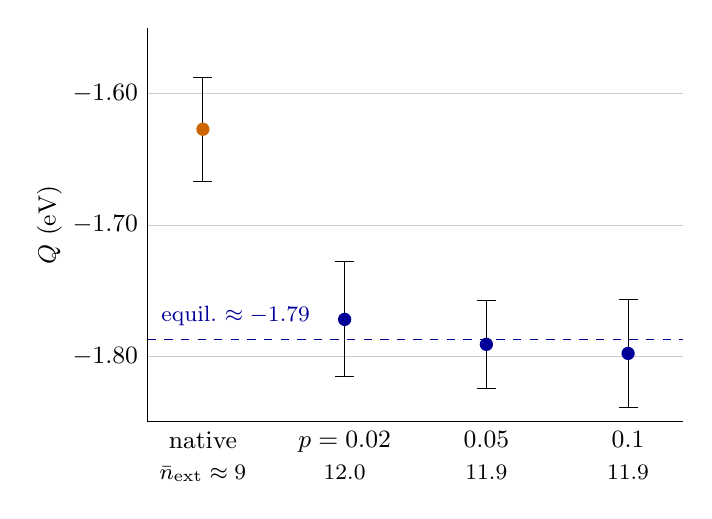
\begin{tikzpicture}[x=1cm,y=1cm,font=\small]
  % y = (Q + 1.85) / 0.06 cm ; x categories at 1.2, 3.0, 4.8, 6.6
  \draw[gray!40] (0.5,0.833) -- (7.3,0.833);
  \draw[gray!40] (0.5,2.5) -- (7.3,2.5);
  \draw[gray!40] (0.5,4.167) -- (7.3,4.167);
  \draw (0.5,0) -- (7.3,0);
  \draw (0.5,0) -- (0.5,5);
  \node[left] at (0.5,0.833) {$-1.80$};
  \node[left] at (0.5,2.5) {$-1.70$};
  \node[left] at (0.5,4.167) {$-1.60$};
  \node[rotate=90] at (-0.75,2.5) {$Q$ (eV)};
  \draw[blue!60!black,dashed] (0.5,1.052) -- (7.3,1.052);
  \node[blue!60!black,anchor=south west] at (0.55,1.1) {\footnotesize equil.\ $\approx-1.79$};
  % error bars and points
  \foreach \x/\lo/\y/\hi in {1.2/3.057/3.717/4.377, 3.0/0.572/1.302/2.032, 4.8/0.428/0.985/1.542, 6.6/0.187/0.870/1.553} {
    \draw (\x,\lo) -- (\x,\hi);
    \draw (\x-0.12,\lo) -- (\x+0.12,\lo);
    \draw (\x-0.12,\hi) -- (\x+0.12,\hi);
  }
  \fill[orange!80!black] (1.2,3.717) circle (2.4pt);
  \foreach \x/\y in {3.0/1.302, 4.8/0.985, 6.6/0.870} { \fill[blue!60!black] (\x,\y) circle (2.4pt); }
  \node[below] at (1.2,0) {native};
  \node[below] at (3.0,0) {$p=0.02$};
  \node[below] at (4.8,0) {$0.05$};
  \node[below] at (6.6,0) {$0.1$};
  \node[below] at (1.2,-0.42) {\footnotesize $\bar n_{\mathrm{ext}}\approx9$};
  \node[below] at (3.0,-0.42) {\footnotesize 12.0};
  \node[below] at (4.8,-0.42) {\footnotesize 11.9};
  \node[below] at (6.6,-0.42) {\footnotesize 11.9};
\end{tikzpicture}
\caption{\label{fig:pscan}Pooled $Q$ for the runs of Table~\ref{tab:pscan}. Native chains started from the bare electron stay near nine external pairs; with the ordered external move every probability reaches the same equilibrium.}
\end{figure}

A standard native run started from the bare electron therefore never reaches equilibrium. Table~\ref{tab:pscan} and Fig.~\ref{fig:pscan} show the effect. Native stays near nine pairs, while an exact ordered external addition and removal at arbitrary positions brings every chain to about twelve. The move respects the ordering invariant and passes L2. In L3 it agrees with fixed native at maxOrder 7 (Table~\ref{tab:maxorder7}), and within $0.8\sigma$ at maxOrder 21 and 51. The energy moves from $-1.627$ to $-1.77\ldots-1.80$~eV, about 9\%, and $\avg{s}$ halves. The result does not depend on $p$ between 0.02 and 0.1.

Two observations confirm that the twelve-pair state is the equilibrium:
\begin{itemize}
\item chains that use the move only during burn-in and then pure fixed native updates stay there ($\bar n_{\mathrm{ext}}=10.9$--11.6, $Q=-1.771\pm0.103$~eV);
\item a five-times longer native run drifts toward it, reaching about 10.6 pairs.
\end{itemize}
The cost per update rises by a factor of about 1.9 at every $p$. This rise is physical: the equilibrium diagrams are larger, so native updates cost more.

\section{Estimators in the low-sign regime}
\label{sec:estimators}

\emph{Pool, then divide.} All chains of a kernel sample the same distribution. The estimator is therefore the pooled ratio
\begin{equation}
R=\frac{\sum_i n_i}{\sum_i d_i},\qquad Q=\frac{R}{\tau_{\max}}-E_{\mathrm{bare}},
\end{equation}
where $n_i$ is the mean numerator and $d_i$ the mean sign of chain $i$. Its variance follows from the chain-level influence $h_i=(n_i-Rd_i)/\bar d$ as $\mathrm{Var}(R)=\mathrm{var}(h)/N$, which we cross-check with a jackknife over chains.

The mean of per-chain ratios is biased when the chain signs scatter. At $T=500$~K they range from 0.01 to 0.26. For a native kernel and a grouped kernel, the mean of per-chain ratios gave $Q=-1.89$ and $-1.72$~eV, an apparent $1.6\sigma$ difference with a variance ratio of 1.38. The pooled estimates, $-1.72$ and $-1.66$~eV, agree.

\emph{Do not trust few batches.} The chain-level variance is heavy-tailed: at full order the top two of 24 chains carried about half of $\mathrm{var}(h)$. At maxOrder 31 and $T=500$~K, $\mathrm{var}(h)$ of the \emph{same} kernel varied by a factor of about five between batches of 16 chains, and the net-efficiency estimate for the general-span move went from 2.35 to 2.62 to 1.08 as batches were added. Variance ratios from fewer than several such batches should not be reported.

\emph{The sign ceiling.} The usual estimate of what sign reduction can gain is $1/\avg{s}^2$. It assumes that removing the sign leaves the other fluctuations unchanged. We measure the gain directly by comparing two per-measurement variances on the same chain, each with its blocking autocorrelation time~\cite{FlyvbjergPetersen1989,Sokal1997}. The first is the ratio-estimator influence $h=s(O-R)/\avg{s}$. The second is the same quantity with the sign set to $+1$, $h_O=O-\avg{O}$. Their ratio bounds the variance reduction of $Q$ that any sign-removal method can achieve (Table~\ref{tab:ceiling}). It is far below $1/\avg{s}^2$, because the sign is fast noise that also decorrelates the slow fluctuations of $O$. In STO, for example, $\tauint(h)=17$ while $\tauint(h_O)=32$.

\begin{table}
\caption{\label{tab:ceiling}Upper bound on the variance reduction of $Q$ from removing the sign, compared with $1/\avg{s}^2$.}
\begin{ruledtabular}
\begin{tabular}{lrrrr}
Case & chains & $\avg{s}$ & $1/\avg{s}^2$ & bound \\
\midrule
LiF electron, $\beta=232$ & 12 & 0.951 & 1.10 & 1.01 \\
STO, $\beta=232$ & 6 & 0.680 & 2.17 & 1.14 \\
LiF hole, $T=500$~K & 3 & 0.096 & 110 & 4.3 \\
\end{tabular}
\end{ruledtabular}
\end{table}

For the published cases no sign-reduction scheme can improve $Q$ by more than 1--14\%. Over 102 production chains of the LiF electron, $\avg{s}=0.944\pm0.002$. A sign-based grouping there could at best gain a factor 1.12, and a four-vertex window grouping would recover about 1.02.

\section{Exact moves and their efficiency}
\label{sec:negative}

Table~\ref{tab:efficiency} lists the levers we tested; all pass L1--L3. We define the net efficiency as the per-step variance ratio divided by the CPU cost ratio, so a value above one is a gain. None exceeds one.

One example shows why. The grouped chain sums phonon modes over the non-crossing lines of a configuration. It raises the sign from 0.68 to 0.91 in STO and from 0.087 to 0.147 for the LiF hole at 500~K, but each step costs several times more.

The moves do mix the slow coordinates faster. With the ordered external move, $\tauint(n_{\mathrm{ext}})$ drops to 56 measurements, and the chain-to-chain sign spread shrinks by a factor of 2--6. However, the variance of $Q$ sits in slow fluctuations of the order and the energy ($\tauint\approx150$--200 measurements), which none of the moves shortens. The slow component of the sign is largely cancelled by the ratio estimator already.

\begin{table}
\caption{\label{tab:efficiency}Net efficiency for $Q$, LiF hole at $T=500$~K, full order, pooled over 12--24 chains per kernel, unless noted. General-span move at $p=0.1$ (0.21 at $p=0.3$). The external move's value is that it removes the bias of Sec.~\ref{sec:equilibration}.}
\begin{ruledtabular}
\begin{tabular}{lr}
Lever & net efficiency \\
\midrule
Grouped measure (non-crossing mode sums) & $\approx0.33$ \\
Mode Rao--Blackwellization & 0.77 \\
Change of momentum (int.; with ext.) & 0.71; 0.86 \\
General-span add/remove & 0.51 \\
New moves in burn-in only & 0.70 \\
Ordered external move, $p=0.1$ & 0.51 \\
Window Rao--Blackwell. (LiF electron) & $\approx1$ \\
\end{tabular}
\end{ruledtabular}
\end{table}

\section{Recommendations}

For users and developers of first-principles DiagMC codes we suggest:
\begin{enumerate}
\item Require single-step round trips (L2) and agreement of independent kernels at low order (L3) for every new or changed update. Of the three defects in Sec.~\ref{sec:defects}, L2 caught the first and L3 the other two.
\item Write down the invariants of the native diagram space before adding moves; an exact move on a larger space silently changes the estimator.
\item In low-sign multiband runs, monitor slow coordinates such as $n_{\mathrm{ext}}$ by quarter of the run, and start from an equilibrated state or use a move that changes them directly.
\item Pool numerators and signs over chains before dividing, and report variance ratios only from several batches.
\item Measure the sign ceiling of Table~\ref{tab:ceiling} before investing in sign reduction; $1/\avg{s}^2$ overstates it by orders of magnitude at low sign.
\end{enumerate}

\section{Conclusion}

A validation ladder applied to the public FEP-DMC code found three defects in the external-phonon updates, a constraint of the native diagram space, and a slow equilibration that biases low-sign multiband runs by about 9\%. The published LiF-electron and STO energies are unchanged within 1--3~meV. Every acceleration lever we tested was exact, but none improved the cost-normalized variance of the energy. The direct sign-ceiling measurement explains why for the published cases: the sign is not where the variance is. The low-sign multiband regime is where an exact grouped measure could still pay off. Doing so would need to include crossing lines and incremental evaluation.

\section*{Code and data availability}
Patches, fixes (as run-time switches), drivers, estimators and the evidence behind every number are in the Future B repository, package \code{future\_b.fepdmc}, releases v1.3.x~\cite{FutureB}. The defects are reported upstream~\cite{UpstreamIssue}.

\begin{thebibliography}{99}
\bibitem{Prokofev1998} N. V. Prokof'ev and B. V. Svistunov, Polaron problem by diagrammatic quantum Monte Carlo, Phys. Rev. Lett. \textbf{81}, 2514 (1998).
\bibitem{Mishchenko2000} A. S. Mishchenko, N. V. Prokof'ev, A. Sakamoto, and B. V. Svistunov, Diagrammatic quantum Monte Carlo study of the Fr\"ohlich polaron, Phys. Rev. B \textbf{62}, 6317 (2000).
\bibitem{Luo2025} Y. Luo, J. Park, and M. Bernardi, First-principles diagrammatic Monte Carlo for electron--phonon interactions and polarons, Nat. Phys. \textbf{21}, 1275 (2025), doi:10.1038/s41567-025-02954-1.
\bibitem{Perturbo2021} J.-J. Zhou, J. Park, I.-T. Lu, I. Maliyov, X. Tong, and M. Bernardi, Perturbo: A software package for ab initio electron--phonon interactions, charge transport and ultrafast dynamics, Comput. Phys. Commun. \textbf{264}, 107970 (2021).
\bibitem{QE2009} P. Giannozzi \emph{et al.}, QUANTUM ESPRESSO: a modular and open-source software project for quantum simulations of materials, J. Phys.: Condens. Matter \textbf{21}, 395502 (2009).
\bibitem{ChristenFox2005} J. A. Christen and C. Fox, Markov chain Monte Carlo using an approximation, J. Comput. Graph. Stat. \textbf{14}, 795 (2005).
\bibitem{FlyvbjergPetersen1989} H. Flyvbjerg and H. G. Petersen, Error estimates on averages of correlated data, J. Chem. Phys. \textbf{91}, 461 (1989).
\bibitem{Sokal1997} A. D. Sokal, Monte Carlo methods in statistical mechanics: foundations and new algorithms, in \emph{Functional Integration}, edited by C. DeWitt-Morette, P. Cartier, and A. Folacci (Plenum, New York, 1997).
\bibitem{FutureB} K. Wong, Future B: exact-corrected delayed acceptance and validation tools for first-principles diagrammatic Monte Carlo, \url{https://github.com/DarrenWongKaWa/future-b} (v1.3.x, 2026).
\bibitem{UpstreamIssue} FEP-DMC issue \#1, \url{https://github.com/yaoluo/FEP-DMC/issues/1} (2026).
\end{thebibliography}

\end{document}
